\documentclass[]{IEEEtran}
\usepackage[utf8]{inputenc}
\usepackage[spanish,es-tabla]{babel}
\usepackage{amsmath}
\usepackage{amsfonts}
\usepackage{amssymb}
\usepackage{graphicx}
\usepackage{cite}
\usepackage{hyperref}
\usepackage{float}

\title{Procesamiento de imágenes utilizando Deep learning y Carla 
Simulator}
\author{ 
Gatica, Isais \\ \small{email: isaiasgatica1@gmail.com} \\ \and 
Saez, Lautaro Andres \\ \small{email: lautaroandressaez@gmail.com } }
\date{}

\providecommand{\keywords}[1]
{
  \small	
  \textbf{\textit{Keywords---}} #1
}

\begin{document}
    \maketitle

    \begin{abstract}
        En este informe se presenta la implementación de una red Pix2Pix capaz de pasar de una imagen RGB a 
        una imagen segmentada donde cada color indica un objeto diferente. Se comenzara desde cero obteniendo el 
        dataset mediante el simulador CARLA para luego poder entrenar la red con una gran variedad de imagenes con 
        diferente clima y vegetación. Finalmente se probara con imagenes reales para analizar la viavilidad de entrenar una 
        red con un simulador y luego ingresarla en el mundo real.
    \end{abstract}

    \keywords{Pix2Pix, CNN, GAN, RNN, NN, YOLO, SOM, CARLA}


    \section{Introducción}

    Con la intención de brindarle inteligencia a un automovil, la primer cuestión es cómo éste se comunica con el mundo y cómo lo interpreta.
    Con el avance de la tecnología las cámaras toman preponderencia como sensores y combinando esta gran fuente de información (la fotografía) con un 
    algoritmo de segmentación las posibilidades de detección y decisión del vehículo parten de una buena base. 

    ¿Pero cómo generar esta segmentación de forma automática y confiable? En los ultimos años, debido a la necesidad de resolver cada vez mas complejos y la posibilidad de utilizar GPU's las redes neuronales han cobrado 
    gran importancia en nuetras vidas, y ya son parte del dia a dia, cosas tan simples como los filtros de Instagram basan 
    su reconocimiento facial en redes neuronales. 

    Las redes permiten resolver problemas que van desde la clasificación de imagenes hasta la conducción autonoma, claro esta 
    que para esto existen diferentes arquitecturas las cuales son expecificas para determinadas tareas, como el procesamiento de imagenes (CNN, GAN, YOLO), 
    procesamiento de texto (RNN), procesamiento de datos (NN).

    La desventaja principal de estos modelos supervisados es la necesidad de una dataset muy bien estructurado y para el cual es necesario 
    el trabajo humano, esta es la tarea mas importante y que si esta mal realizada el red no tendra un desempeño correcto.

    Aquí es donde nace el uso de simuladores. En el paper \textit{Driving to Safety} de las autoras \textit{Nidhi Kalra} y \textit{Susan M. Paddock}, se 
    plantean la siguiente cuestión ``los vehículos autónomos deberán ser conducidos cientos de millones de millas y, a veces, cientos de miles de millones de millas
    para hacer afirmaciones estadísticamente confiables sobre la seguridad''. Esto conlleva obviamente muchos gastos y riesgos, lo que un simulador reduce de gran 
    manera, no solo para la creación del dataset si no tambien para el posterior testeo de la conducción autonoma. 



    \section{Materias y metodos}

    En esta sección se detallan los recientes avances en los campos de interes.


    \subsection{CARLA}

    CARLA \cite{CARLA-Simulator} es un simulador de conducción el cual posee una API para Python lo que 
    permite de forma sencilla obtener datos del entorno. Esto permite una gran simpleza 
    a la hora de crear dataset o probar modelos de AI.
    
    CARLA cuenta con una gran variedad de sensores como GPS, LiDAR, camaras RGB, camaras de segmentación semantica, etc.
    También posee un ambiente muy variado, permiendo variaciones en la neblina, la hora del día e incluso el clima.

    \subsection{Deep Learning}

    Las redes neuronal son muy utilizadas en el campo de la minería de datos, debido a 
    su gran versatilidad. Dentro de este mundo existen 2 grandes tipos de entrenamientos 
    para los supervisados que dada una entrada $X$ se conoce la salida deseada $Y$ y 
    otros casos los algoritmos no supervisados como los modelos de Q-learning o los mapas autoorganizados (SOM).
    En este proyecto se opto por un entrenamiento supervisado.

    

    Para el modelado de la red neuronal se utilizó un modelo llamado Pix2Pix \cite{Pix2Pix}.
    El cual pertime dada una imagen de entrada $X$ obtener una imagen de salida $Y$.

    Este modelo consta de $2$ redes separadas, la primera se denominada el generador Fig.\ref{fig:generator}
    el cual deberá aprender a segmentar la imagen semanticamente. Y la segunda se llama el discriminador Fig.\ref{fig:discr}
    este se encarga de correguir al generador aprendiendo cuando una salida es "realista". 
    Llamaremos salida "realista" a aquella imagen que cumpla el objetivo esperado, en este caso sería una imagen segmentada 
    de coherente.
    
    \begin{figure}
        \centering
        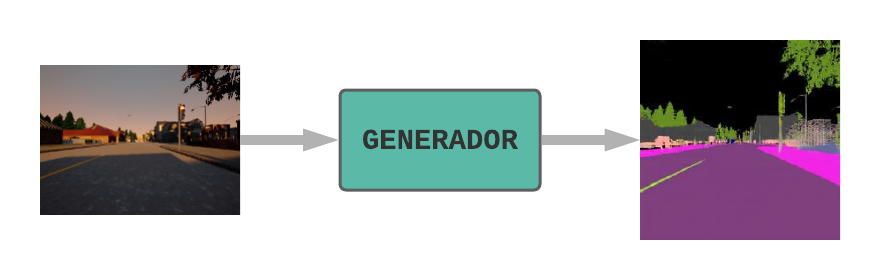
\includegraphics[width=.4\textwidth]{Imgs/Generador.png}
        \caption{Esquema de la red generativa.}
        \label{fig:generator}
    \end{figure}

    \begin{figure}
        \centering
        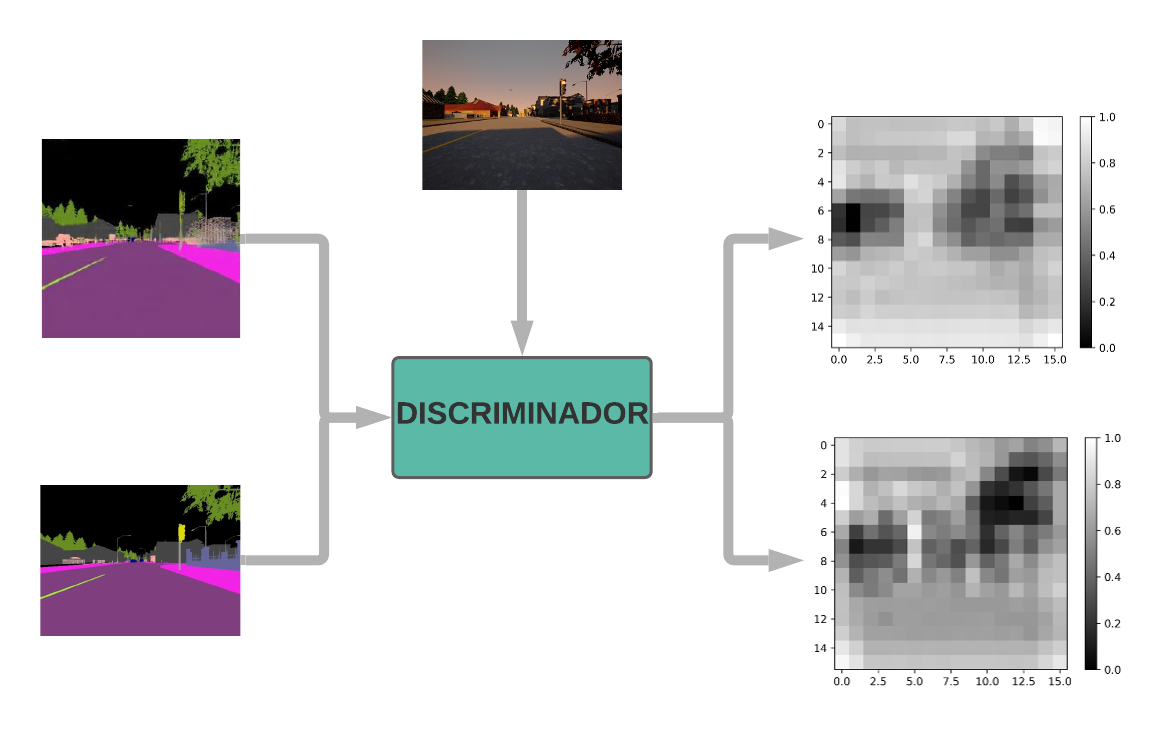
\includegraphics[width=.4\textwidth]{Imgs/Discriminador.png}
        \caption{Esquema de la red discriminativa.}
        \label{fig:discr}
    \end{figure}
    


    \subsubsection{Generador}

    El generador cuenta con una arquitetura denomina U-net \cite{U-Net}, la cual tiene 
    la cual posee una muy buena eficiencia debido a los bypass que existen entra las capas de convolución y 
    las capas de deconvulición. Con la finalidad de comprender de forma mas sencilla se puede observar 
    en la Fig.\ref{fig:u-net} dicha arquitectura.

    \begin{figure}
        \centering
        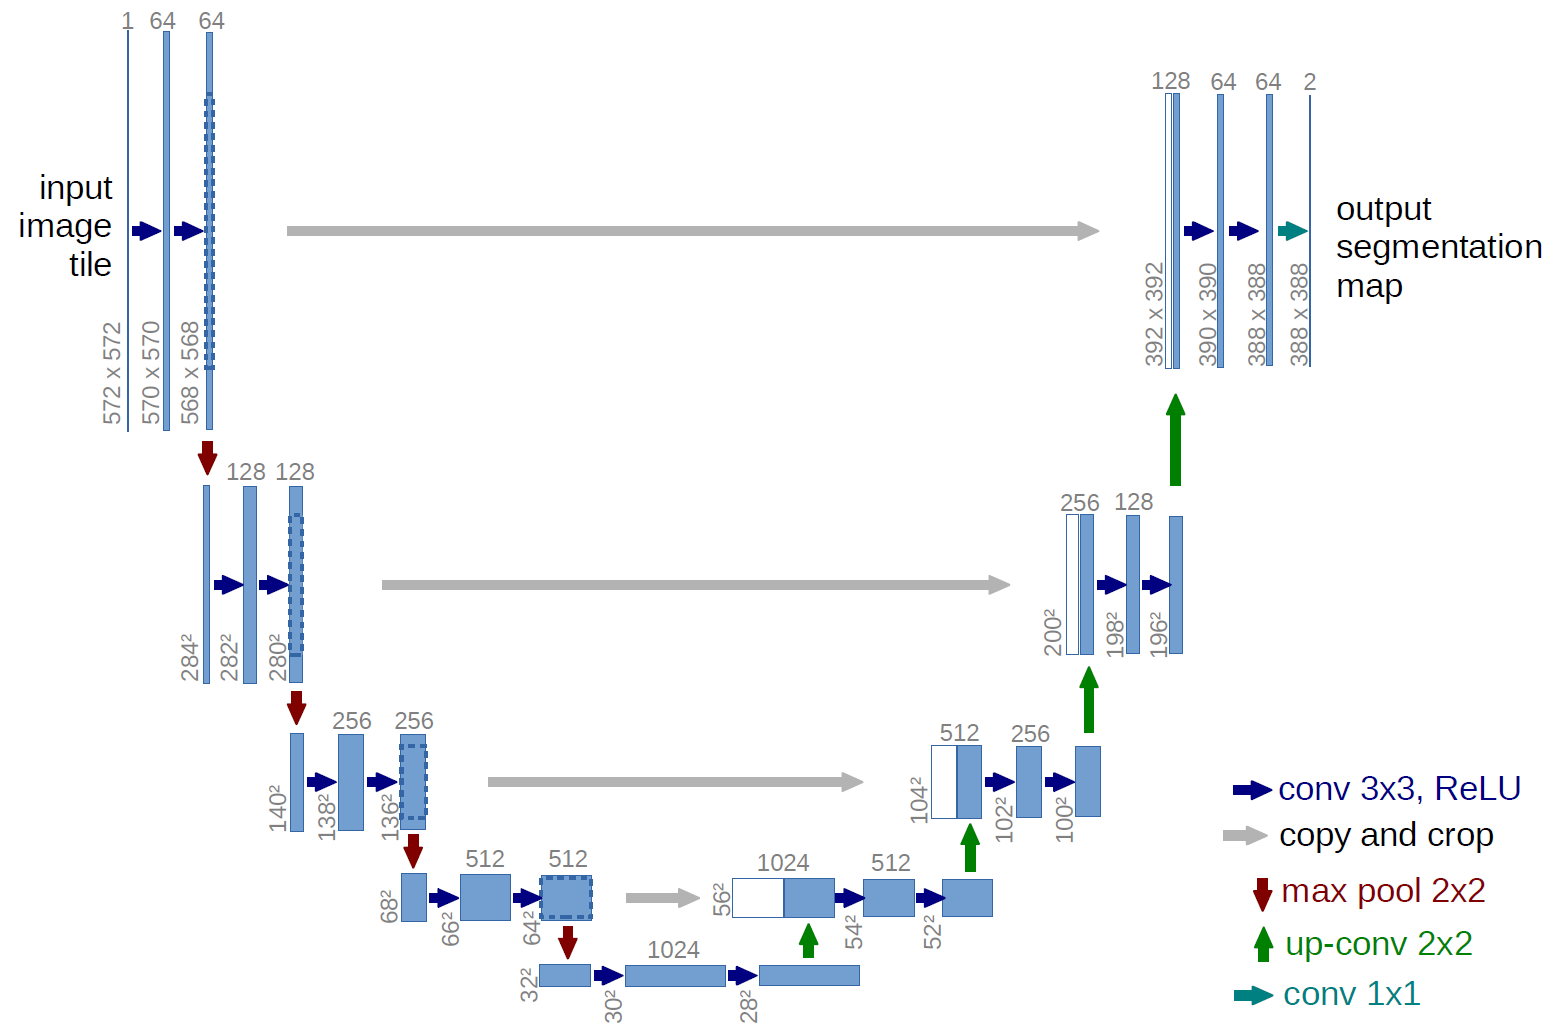
\includegraphics[width=.4\textwidth]{Imgs/u-net-architecture.png}
        \caption{Arquitectura de una U-net.}
        \label{fig:u-net}
    \end{figure}

    El error del generador es cuantizado por la red discriminativa.

    \subsubsection{Discriminador}

    El discriminador posee una arquitectura mucho mas sencilla, la cual consta de $6$ capas de convolución.
    Esto se debe a que la salida representa que tan realista es un segmento de la imagen de entrada. 
    El error del discriminador se cuantiza mediante una entropía cruzada. Ya que 
    se propone que siempre que le entre una imagen del generador la salida debe ser una matriz de $0$, ya que 
    esta imagen no es del dataset, mientras que cuando la entrada sea una imagen del dataset el resultado debe ser un $1$. 
    
    Estodesemboca en una pelea entre en generador ya que debe aprender a engañar al discriminador 
    y el discriminador que debe lograr siempre reconocer que la imagen $\hat{Y}$ es totalmente falsa, ya que es una 
    creación de la red generativa.
 
    \subsection{Preporcesado de los datos}

    Un paso fundamental para trabajar con algoritmos de imagenes es pasar del domininio $[0;255]$ a 
    un dominio mas acotado, para este trabajo se utilizo el domino de $[-1;1]$. De esta forma se logra 
    una mayor eficiencia computacional.

    Debido al tamaño de las imagenes es recomendable hacer un resize a dimensiones mas pequeñas 
    para disminuir el uso de RAM cuando son cargadas en memoria y el uso de GPU al realizar las convoluciones. En 
    este caso las imagenes de entrada y de salida son redimensionadas a $256x256$.

    \subsubsection{Random jitter}

    El \textit{random jitter} es un proceso por en el cual se busca realizar un aumentado
    del dataset, esto disminuye la posibilidad de experimentar \textbf{overfitting}. 
    Este proceso cuenta de $2$ pasos:

    \begin{itemize}
        \item[Crop] Se realiza un resize a $286x286$ para luego realizar un recorte a $25x256$.
        \item[Flip] De forma aletoria con probabilidad $0.5$ se realiza un rotación de $180^\circ$. 
    \end{itemize}

    Debido a que es utiliza en algoritmos supervisados es necesario aplicar 
    el \textit{random jitter} tanto a la imagen de entrada como a la de salida,
    para ello se hace un stack de las mismas como se observa en la Fig.\ref{fig:random-jitter}.

    \begin{figure}
        \centering
        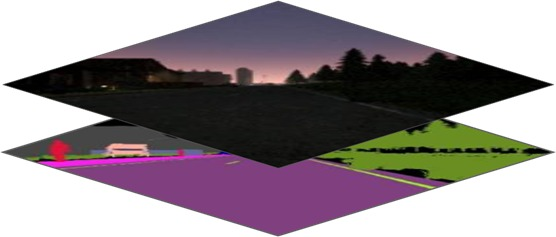
\includegraphics[width=.4\textwidth]{Imgs/stack-random-jitter.jpeg}
        \caption{Visualización del stack previo al random jitter.}
        \label{fig:random-jitter}
    \end{figure}

    En la Fig.\ref{fig:crop-flip} se observa el proceso de random jitter completo.

    \begin{figure}
        \centering
        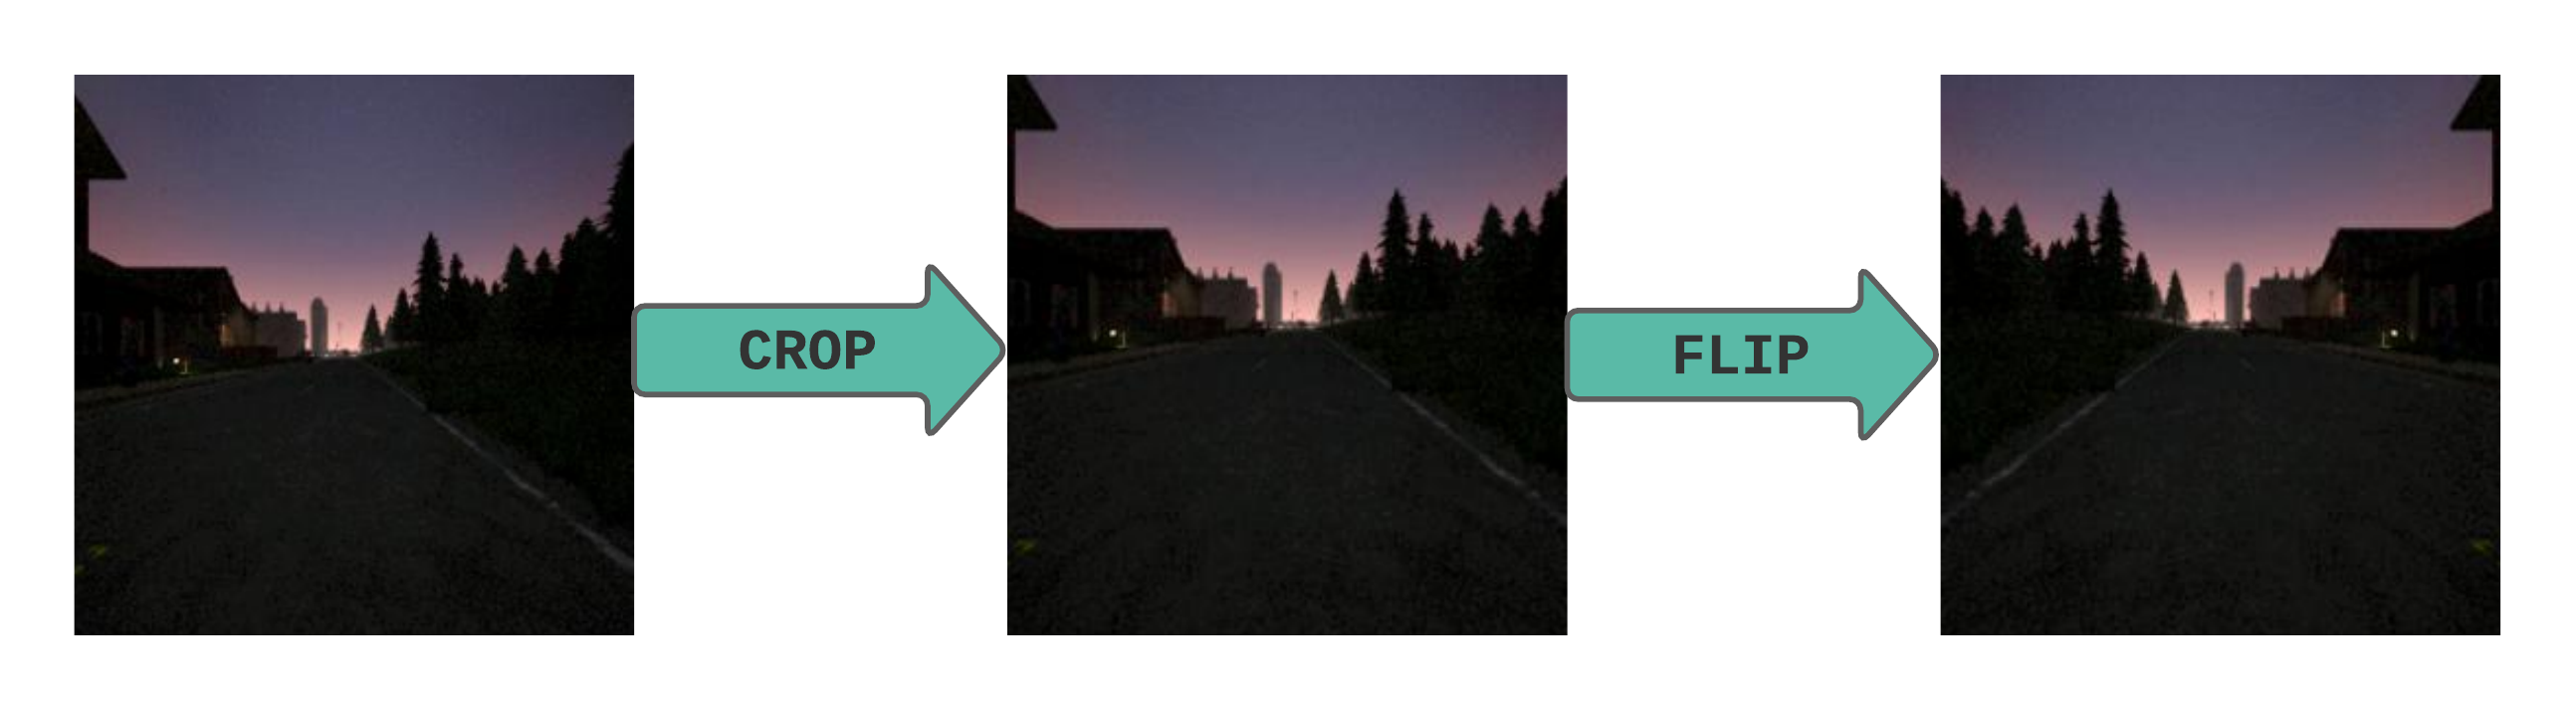
\includegraphics[width=.4\textwidth]{Imgs/in_crop_flip.png}
        \caption{Visualización del random jitter.}
        \label{fig:crop-flip}
    \end{figure}

    \section{Propuesta}

    Se propone realizar una red neuronal utilizando la arquitectura Pix2Pix que 
    aprenda a segmentar semanticamente una imagen. Adicionalmente el 
    dataset utilizado será obtenido mediante el CARLA permitiendo de esta forma 
    pasar por todo el trayecto del diseño de una red que resuelve un nuevo problema. 
    Este proceso consta de 

    \begin{enumerate}
        \item Definir la arquitectura a utilizar.
        \item Crear un dataset util para solucionar el problema.
        \item Entrenar la red.
        \item Testear el rendimiento de la misma.
        \item Realizar mejoras a la arquitectura para obtener alguna de las siguientes ventajas: 
            \subitem Mayor velocidad de procesado.
            \subitem Mejor rendimiento. 
            \subitem Eliminar el overfitting o underfitting si existiera.
        \item Repetir los pasos anteriores hasta lograr un resultado satisfactorio.
    \end{enumerate}

    \section{Pruebas y resultados}

    Se presentara de forma ordena todas las etapas del proyecto. 
    Debido a la cantidad de imagenes utilizadas no es posible presentarlas a todas, por ello 
    se relizaran analisís particulares para algunos casos de interes.

    \subsection{Obtención del dataset}

    Para obtener el dataset se colocaron una camara RGB y una camara de segmentación semántica
    \cite{CARLA-Sensors-Reference}, ubicadas en la misma posición. Se recolectaron los datos 
    cada 5 segundos. Las condiciones climaticas utilizadas fueron aletorias, lo que se logra
    obtener un dataset mucho mas variado, una representación de este puede observase en 
    Fig.\ref{fig:dataset}.

    \begin{figure}
        \centering
        %\includegraphics[width=.5\textwidth]{Imgs/tar_crop.jpg}
        \caption{Imagenes de muestra del dataset}
        \label{fig:dataset}
    \end{figure}

    Para lograr un manejo autónomo del vehículo se utilizó el autopilot \cite{CARLA-Documentation}. 
    Con la finalidad de aumentar la variedad de imágenes se utilizaron todos los mapas posibles y 
    se adicionaron otros vehiculos autónomos junto a personas. Aunque debido 
    a limitaciones de hardware solo se pudieron ingresar 20 personas, lo cual 
    provocó una deficiencia en la detección de personas de la red Pix2Pix. 

    \subsection{Entrenamiento de la red}

    Como fue mencinado en el marco teoríco el modelo implementado se denomina Pix2Pix \cite{Pix2Pix}.
    Se utilizó como entrada la imagen de la camara RGB y la salida será una imagen segmentada, para ello se utilizó
    el dataset obtenido con el simulador de \textbf{CARLA} el cual posee 8000 imagenes. 

    \subsubsection{Tratamiento de las imagenes}

    Para evitar problemas en el entrenamiento de la red es muy usual llevar los valores de cada canal al 
    intervalor $[-1;1]$, esto evita problemas de continuidad en red. Luego 
    se procede a aplicar un \textit{random jitter}.

    El dataset fue dividido en 2 partes una utilizada para el entrenamiento, aproximadamente el $80 \% $ de las imagenes y 
    otra parte para el testing de la red utilizando el $20 \%$ restante, siguiendo el principio de Pareto.

    \subsubsection{Entrenamiento}

    Para realizar el entremiento se utlizó el dataset de testin, aproximadamente 6400 imagenes, 
    y se realizon 400 iteraciones a la red para lograr un mejor desenpeñó. 
    
    En la Fig.\ref{fig:results}
    se muestra una comparación para $1$ imagen del dataset de testing luego de la primera iteración 
    y al finalizar el entrenamiento.
    Puede observarse que existieron grandes mejoras sobre todo en la zona de la palmera
    donde al finalizar el entrenamiento es posible observar los detalles de la misma.
    Aunque cabe destacar que debido a la poca cantidad de señales de trafico en el dataset
    se observa que si bien reconoce la estructura del semaforo no es capaz de utilizar el color 
    adecuado.

    \begin{figure}[htb]
        \centering
        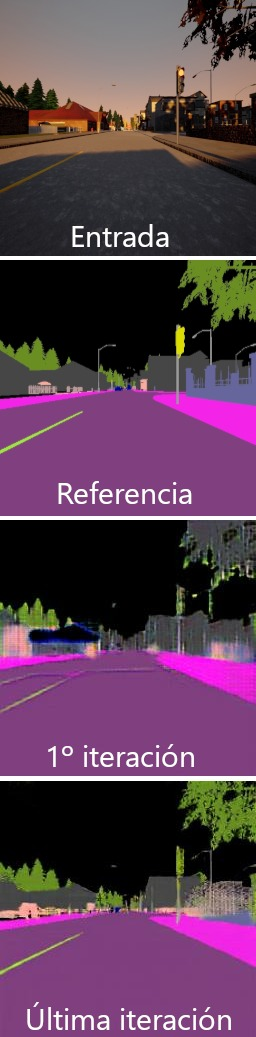
\includegraphics[width=.25\textwidth]{Imgs/results.jpeg}    
        \caption{Imagen del dataset de testing.}
        \label{fig:results}
    \end{figure}

    Al analizar otro imagen del dataset la cual se observa en la Fig.\ref{fig:person_image}
    {COMPLETAR!!!}

    \subsection{Imágenes reales}
    En la siguientes imágenes se observa el desempeño de la red al utilizar imágenes reales de un dataset público. 
    \begin{figure}[htb]
        \centering
        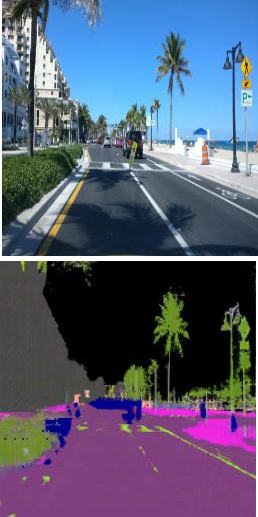
\includegraphics[width=.25\textwidth]{Imgs/PalmeraRGBSEM.png}    
        \caption{Primer prueba con imagen real.}
        \label{fig:real-results}
    \end{figure}
    \begin{figure}[htb]
        \centering
        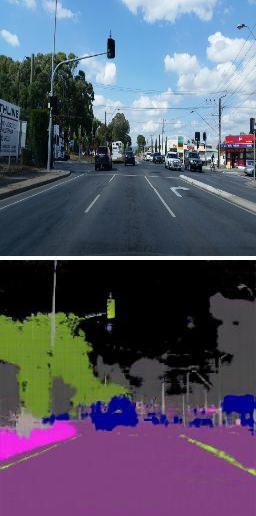
\includegraphics[width=.25\textwidth]{Imgs/SemaforoRGBSEM.png}    
        \caption{Segunda prueba con imagen real.}
        \label{fig:real-results2}
    \end{figure}

    \section{Conclusiones}
    
    Al observar la Fig.\ref{fig:resultados2} y el video asociado, se puede concluir que los resultados son precisos, al compararlos con la
    imagen semántica obtenido del simulador. Existen ciertos detalles como las paradas de colectivo, señales de tránsito o peatones que no los 
    reconoce y, si lo hace no le asigna el color adecuado. 
    Sin embargo en las regiones mas significativas como los autos, calles o veredas
    logra un desempeño aceptable. Por otro lado, en las Fig.\ref{fig:real-results} y Fig.\ref{fig:real-results2} donde se analiza a la red con imágenes reales,
    se observa que existen más errores a la hora de segmentar. Hay regiones que no se delimitan correctamente y/o colores que no son 
    los correctos. Por ejemplo la mancha azul en los arbustos de la primera imagen. Las regiones mas significativas en este caso logran un 
    resultado parcialmente aceptable que aún así se podrían utilizar para darle redundancia al sistema. Lo más probable es que estos 
    errores se deban a la diferencia de iluminación y cantidad de detalles que tiene una imagen real en comparación con las imágenes 
    del simulador.

    \subsection{Ventajas}

    A continuación se nombrarán algunas ventajas de realizar la segmentación semántica, en particular con un simulador y una red Pix2Pix. 
    Ordenadas según importancia decreciente:
    
    \begin{enumerate}
        \item Posibilidad de reconocer objetos o zonas de una forma
        mucho mas sencilla. 
        \item Al utilizar un simulador la principal ventaja recae en la posibilidad de crear un dataset con el mínimo esfuerzo humano, tiempo y costo monetario.
        \item Gran flexibilidad de simular situaciones externas o propias del
        vehículo mientras se recolectan datos. Permitiendo simular situaciones anómalas.
        \item Al utilizar redes neuronales no existe una etapa de diseño de descriptores, ya que estos son obtenidos por la red.
        \item Reducción del tiempo de procesado de información.
        \item Las imágenes semánticas ocupan menos espacio en memoria que su equivalente en RGB.
    \end{enumerate}
    
    \subsection{Desventajas}
    
    Por otro lado al analizar las desventajas de este modelo con el mismo criterio obtenemos:
    
    \begin{enumerate}
        \item Existe una diferencia significativa entre el entorno simulado y el real.
        \item Limitaciones de las computadoras actuales para realizar procesos de simulación y train en forma simultanea.
        \item A la hora de implementar la red neuronal las desventajas recaen en la cantidad de tiempo necesario para entrenarlas, el costo computacional 
        y en particular ... %Poner eso de que no se puede editar mucho, como si fuera un sistema cerrado
        \item Para problemas de alta complejidad y modelos de gran densidad es necesario datasets de gran tamaño.
        \item Tiempo de generado del dataset.
    \end{enumerate}


    Por último, como conclusión general cabe destacar que este tipo de prácticas son muy importantes y utilizadas en la actualidad. Las redes neuronales 
    están revolucionando la forma de trabajar y pensar en distintos ámbitos. Debido a esto nace la necesitades de minar datos, 
    su coste es un gran trabajo humano durante largos periodos de tiempo. Esto causa un gran gasto monetario en las empresas que se 
    dedican a este rubro. Por ello es importante el avance de los simuladores para lograr obtener datasets más económicos.


    \bibliographystyle{IEEEannot}
    \bibliography{biblio}
\end{document}